\chapter{\tsPEG{} documentation}
\label{tspegdocs}

\section{tsPEG : A PEG Parser Generator for
TypeScript}\label{tspeg-a-peg-parser-generator-for-typescript}

\emph{tsPEG} is a PEG Parser generator for TypeScript. \emph{tsPEG}
takes in an intuitive description of a grammar and outputs a fully
featured parser that takes full advantage of the TypeScript type system.

\subsection{Installation}\label{installation}

\texttt{tspeg} can be installed by running

\begin{verbatim}
npm install -g tspeg
\end{verbatim}

\subsection{Features}\label{features}

\begin{itemize}

\item
  Fully featured PEG support, more powerful than CFGs.
\item
  Infinite lookahead parsing, no restrictions.
\item
  Regex based lexing, implicit tokenisation in your grammar
  specification.
\item
  Tight typing, generates classes for all production rules,
  differentiable using discriminated unions.
\end{itemize}

\subsection{CLI Usage}\label{cli-usage}

The CLI invocation syntax is as follows

\texttt{tspeg\ \textless{}grammar-file\textgreater{}\ \textless{}output-file\textgreater{}}

This generates a TypeScript ES6 module that exports a parser class, as
well as classes that represent your AST.

\subsection{Parser Usage}\label{parser-usage}

The parser exports a \texttt{parse} function that accepts an input
string, and returns \texttt{ParseResult} object like this

\begin{verbatim}
class ParseResult {
    ast: START | null;
    err: SyntaxErr | null;
}
\end{verbatim}

If the err field is non-null, then a syntax error was found, otherwise
the AST is stored in the \texttt{ast} field.

\subsection{Grammar Syntax}\label{grammar-syntax}

\emph{tsPEG} grammars are specified with a simple syntax, similar to the
classic EBNF syntax.

Grammars are composed of a sequence of rules, each rule defines what
text that it should match, using regex literals, names of rules, and
powerful \protect\hyperlink{operators}{operators} like
\texttt{\textbar{}} for choice.

Each rule is defined by a name, followed by a \texttt{:=} sign and then
a ``rule description''. Rule descriptions are easiest seen by example
here:

\begin{verbatim}
hello := 'Hello '
helloWorld := hello 'World'
helloChoice := hello 'Mars' | helloWorld
\end{verbatim}

\begin{itemize}

\item
  The first line defines a rule \texttt{hello} which matches the string
  `Hello' directly.
\item
  The next line defines the rule \texttt{helloWorld}, this rule first
  matches our first rule \texttt{hello}, then matches the string
  `World', i.e it matches the string ``Hello World''.
\item
  The third line uses the \texttt{\textbar{}} operator to make a choice
  between two options.

  \begin{enumerate}
  \def\labelenumi{\arabic{enumi}.}
  
  \item
    First this rule will try to match the left hand side of the
    operator: \texttt{hello\ \textquotesingle{}Mars\textquotesingle{}},
    which as before will first match the rule \texttt{hello}, then the
    regex literal \texttt{Mars}.
  \item
    If this left hand side fails, we move on to trying the right hand
    side, which is just a reference to the \texttt{helloWorld} rule. In
    practice this means it either matches ``Hello World'' or ``Hello
    Mars''
  \end{enumerate}
\end{itemize}

\emph{tsPEG} \textbf{starts parsing with the first rule in the grammar}
so to match the \texttt{helloChoice} rule we should either move it to
the start or defined a \texttt{start} rule that points to it like this:

\begin{verbatim}
start := helloChoice
hello := 'Hello '
helloWorld := hello 'World'
helloChoice := hello 'Mars' | helloWorld
\end{verbatim}

Putting this grammar into a file called ``grammar.peg'' and running
\texttt{tspeg\ grammar.peg\ parser.ts} we get our parser for this simple
grammar in the file ``parser.ts''. We can compile this (target at least
es2015) and load it into NodeJS to test it.

\begin{figure}[ht]
\centering
    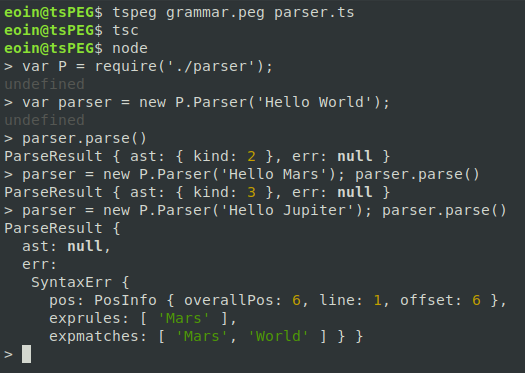
\includegraphics[scale=0.7]{src/app1assets/example1.png}
\caption{Example 1}
\end{figure}

As you can see we get \texttt{null} error for `Hello World', and `Hello
Mars', this means the match was successful. But when we try `Hello
Jupiter' we get an error object, and it lists the location of the error,
and the expected matches at that location, namely `Mars' or `World'. You
can see more about errors in the
\protect\hyperlink{syntax-errors}{Syntax Error section.}

Notably the \texttt{ast} field of the parse result is empty. This is
because we haven't told \emph{tsPEG} what elements of the grammar we
would like to be returned. When we write a rule definition, we can
specify the fields we'd like to save in the AST by assigning them with
an \texttt{=} sign. For example, say we want to match a string that's
the sum of 2 numbers, e.g. ``2+3'', ``123+456'', we'd like to save both
side of the sum in our AST, we can do this by writing a grammar like the
following. \emph{Note that we had to write `\textbackslash{}+' to escape
the `+' symbol as the `+' symbol has special meaning in regex}.

\begin{verbatim}
sum := left=num '\+' right=num
num := '[0-9]+'
\end{verbatim}

Running \emph{tsPEG} on this input and testing the parser in node we can
see that the parser result has saved the left and right numbers of our
sum. Note that we didn't have to assign the result of the
\texttt{{[}0-9{]}+} rule in the \texttt{num} rule. This is because rules
that are just references to other rules are saved implicitly.

\begin{figure}[ht]
\centering
    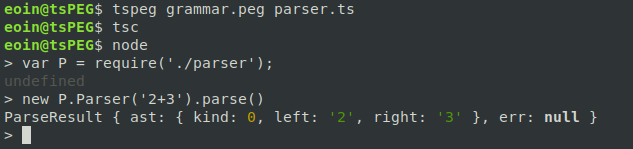
\includegraphics[scale=0.7]{src/app1assets/sum.png}
\caption{Sum example}
\end{figure}

Now that we have saved the numbers of our sum, it's easy to write a
program to compute the result of adding the numbers. Each rule that
assigns results to the AST is exported as a class or interface with the
same name as the rule, so we can just import the \texttt{sum} interface
from the parser to write our function. For this grammar we get an
interface like:

\begin{verbatim}
interface sum {
    left: string;
    right: string;
}
\end{verbatim}

Allowing us to write our calculator function like:

\begin{verbatim}
import { sum } from "./parser";

export function add(ast: sum): number {
    return parseInt(ast.left) + parseInt(ast.right);
}
\end{verbatim}

Calling this file ``calc.ts'' we can use it to calculate our sums:

\begin{figure}[ht]
\centering
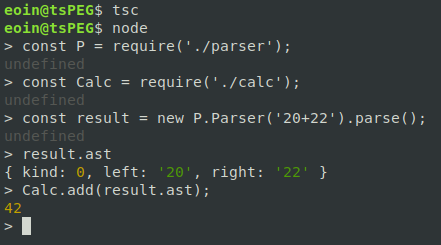
\includegraphics{src/app1assets/calc.png}
\caption{Calc screenshot}
\end{figure}

We can also use \protect\hyperlink{computed-properties}{computed
properties} to calculate the result of the sum during the parsing
process.

\hypertarget{operators}{\subsection{Operators}\label{operators}}

\emph{tsPEG} supports a set of powerful operators to build complex
grammars. The only operator we have seen so far is the
\texttt{\textbar{}} operator, which allows us to make choices between
two rule expressions, however there are many more.

\begin{itemize}
\item
  The \texttt{?} operator is used to make a match optional. For example
  in the rule

\begin{verbatim}
rule := 'I ' 'really '? 'love tsPEG'
\end{verbatim}

  The match for the `really' string has been marked optional, so this
  rule can match either ``I really love tsPEG'', or ``I love tsPEG''.
\item
  The \texttt{+} operator matches 1 or more copies of the match it's
  applied to, for example:

\begin{verbatim}
rule := 'It\'s a ' 'long '+ 'way away'
\end{verbatim}

  This rule matches ``It's a long way away'', ``It's a long long way
  away'', etc. for any amount of ``long''s that's not 0. When this
  operator is used, a list of results is attached to the AST.
\item
  The \texttt{*} operator is the same as the \texttt{+} operator but it
  allows zero matches.
\item
  The \texttt{!} is called the ``\emph{negative lookahead}'' operator,
  and it does exactly what it says on the tin. This operator inverts the
  result of the match, meaning you can specify a rule by what it should
  not match. For example the rule
  \texttt{rule\ :=\ \textquotesingle{}The\ banned\ word\ is\ \textquotesingle{}\ !\textquotesingle{}Macbeth\textquotesingle{}}
  This will match the phrase ``The banned word is X'' for any value of
  X, except when X is `Macbeth'
\item
  The \texttt{\&} operator is called the ``\emph{postitive lookahead}''
  operator, this operator will change a match so that it will test for
  the match, and fail if it doesn't work, but it will not consume the
  input. This allows you to lookahead at what comes next in the string,
  but not to consume it.
\end{itemize}

\hypertarget{syntax-errors}{\subsection{Syntax
Errors}\label{syntax-errors}}

A \texttt{SyntaxErr} object is composed of two fields, a \texttt{pos}
field with the position of the error, and \texttt{expmatches} which
contains a list of expected matches.

\begin{verbatim}
class SyntaxErr {
    pos: PosInfo;
    expmatches: string[];
}
class PosInfo {
    overallPos: number;
    line: number;
    offset: number;
}
\end{verbatim}

\hypertarget{computed-properties}{\subsection{Computed
Properties}\label{computed-properties}}

As well as assigning parsing results to variables and storing them on
the AST, \emph{tsPEG} also allows you to create \textbf{computed
properties}, which are fields on the AST that are computed when the
parser is run.

Computer properties are added to a rule by appending a new expression
after the rule description like

\begin{verbatim}
.<propertyname> = <type> { <code to calculate property> }
\end{verbatim}

Returning to our sum example from earlier we had a grammar to match
strings like ``2+3'', ``40+200'' etc.

\begin{verbatim}
sum := left=num '\+' right=num
num := '[0-9]+'
\end{verbatim}

We can add computed properties to this to compute the value of this sum
at parse time, instead of writing our own function to do it after. First
we add a computed property to \texttt{num} to store the value of the
number:

\begin{verbatim}
sum := left=num '\+' right=num
num := literal='[0-9]+'
       .value = number { return parseInt(this.literal); }
\end{verbatim}

As you can see we've assigned the text match to the field
\texttt{literal}, and added a computed property called \texttt{value}
which is the \texttt{literal} field parsed as an integer.

Now we can add a computed property to \texttt{sum} to do the arithmetic,
this is very simple

\begin{verbatim}
sum := left=num '\+' right=num
       .sum = number { return this.left.value + this.right.value }
num := literal='[0-9]+'
       .value = number { return parseInt(this.literal); }
\end{verbatim}

We use the computed property of the \texttt{num} rule to compute our
\texttt{sum} property. Let's see this in action! Let's try and parse the
string ``240+100''.

\begin{figure}[ht]
\centering
    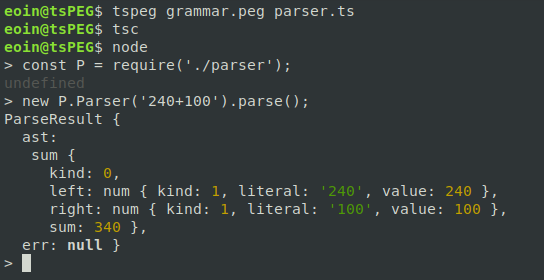
\includegraphics[scale=0.7]{src/app1assets/computed.png}
\caption{Computed property}
\end{figure}

As you can see the AST has a field called \texttt{sum} with the correct
value of 340 in it. The \texttt{left} and \texttt{right} also have their
computed \texttt{value} properties of 240 and 100.

\subsection{Header}\label{header}

The introduction of computed properties means that now you might want to
import some types or functions into your parser. Luckily you can specify
a header in the file that will be inserted directly into the generated
parser. Anything at the top of the grammar file between two lines of
three dashes \texttt{-\/-\/-} will be inserted straight into the
generated parser, allowing you to write grammars like

\begin{verbatim}
---
import { myFunc, myType } from "./mypackage";
---
rule := hello='Hello World'
        .value = myType { return myFunc(this.hello); }
\end{verbatim}
